\section{Artificial Neural Networks}
With this chapter, the second part of the course begins.

\subsection{Problem}
We have $f: X \xrightarrow[]{}Y$, a dataset $D=\{(x, t)\}$, a model $\hat{f} (x; \Theta)$, an error function $E(\Theta)$, we want to minimize $\Theta^{*} = argmin E(\Theta)$ and predict the value of $x' \not\in D,\ \hat{f}(x', \Theta)$. The minimization will be tone through Iterative Linear Descent.

What is different from the previous models? $\hat{f}$ is non-linear both in the parameters and the dataset. So, NN provide non linear models in the set of parameters.

The second important aspect is that NN has the advantage that you don't have to specify a kernel. This is because kernels are automatically learned.

Alternative names are \textbf{Feedforward neural network} or \textbf{Multilayer perceptrons}. NN are function estimators and learn parameters so that the function \textbf{f} that they are learning approximates well the unknown function $f$.

\subsubsection{Inspiration}
NN were inspired by what we know of our brain. Note that they are not a model of the brain, but only comprehends some insights. Outputs can be seen as an array of units (neurons) activation based on the connections with the previous units. Feedforward NN are organized in layers, where each layer contains a set of neurons and each one is connected to every unit of the layer that follows. Information flows without any loop from the input to the output, passing through the hidden units.
\begin{equation}
    f(x; \Theta) = f^{3}(f^{2}(f^{1}(x; \Theta^{1}); \Theta^{2}); \Theta^{3})
\end{equation}
where $f^{i}$ is the i-th layer and $\Theta^{i}$ is the corresponding parameters.\\

The power of FNN is based on the fact that we don't have to handcraft kernels or to use a known one.\\
\subsection{XOR problem}
Consider the problem where we have a dataset: $D=\{((0, 0)^{T}, 0), ((0, 1)^{T}, 1), ((1, 0)^{T}, 1), ((1, 1)^{T}, 0),\}$ and we want to use the linear regression using the Mean Square Error (MSE). We can instantly notice that the datast is not linearly separable. If we use a linear model with a linear kernel it will not work. We could try a kernel, but with FNN we don't need to handcraft it.

We can build a two-layer network with two units as input layer, two units as hidden layer and one unit as output layer. We also have to define \textbf{activation function} These functions are present in any hidden layers as well as in the output layer. We can chose a different activation function for each layer. For this example we can use a \textbf{ReLU (rectified linear unit)} for the hidden layer and a linear activation function for the output layer.\\
\textbf{ReLU}: The ReLU units is a function that returns: $f(z)= max(0, z)$.\\
The i-th neuron of the hidden layer will have the form of:
\begin{equation}
    h_{i} = ReLU\left((w_{i,1}, w_{i,2})^{T} \begin{pmatrix} x_{i,1} \\ x_{i,2} \end{pmatrix} + w_{i,0}\right)
\end{equation}
we can then organize as a column vector each unit $h_{i}$ of the layer and rewrite as:
\begin{equation}
    h = \begin{pmatrix} h_{1} \\ h_{2}  \end{pmatrix} = ReLU\left(\begin{pmatrix} w_{1,1} & w_{1,2} \\ w_{2,1} & w_{2,2} \end{pmatrix} \begin{pmatrix}
        x_{1} \\ x_{2}
    \end{pmatrix} + \begin{pmatrix}  w_{1,0} \\ x_{2,0}
    \end{pmatrix}\right) = ReLU\left( W^{T}x + W_{0} \right)
\end{equation}

and so the ourpur of the model $y$ is
\begin{equation}
    y = w^{T} h + w_{0} = w^{t}ReLU\left( W^{T}x + W_{0} \right) + w_{0}
\end{equation}
We can now choose an error function. For instance, can use the MSE and minimize.

\subsection{Cost Function}
A model implicitly defines a conditional distribution $p(t| x, \Theta)$. This cost function is the Maximum likelihood principle (\textbf{cross-entropy}).
\begin{equation}
    J(\Theta) = E_{x, t\sim D} \left[-ln(p(t|x; \Theta))\right]
\end{equation}
For example we can assume the function to be a Gaussian distribution and hence use it to estimate and minimize the loglikelihood.

\subsection{Output units}
The choice of the loss function is related to the problem that we are modeling and to the output units of the network.
\begin{enumerate}
    \item Regression
    \item Binary Classification
    \item Multi-classes classification
\end{enumerate}

\textbf{Regression} \\
linear units: identity activation function.\\
\begin{equation}
    y = W^{T}h + b
\end{equation}
use a Gaussian distribution noise model
\begin{equation}
    p(t|x) = N(t|y, \beta ^{-1})
\end{equation}
\textit{Cost function} = maximum likelihood that is equal to the mean squared error.

\textbf{Binary classification} \\
Sigmoid units: sigmoid activation function.\\
The likelihood corresponds to a Bernoulli distribution.
\begin{equation}
\begin{multlined}
    J(\Theta) = E_{x, t \sim D}\left[-ln(p(t|x))\right] \\
    \textbf{where } -ln (p(t|x)) = softplus ((1 - 2t)\alpha) \\
    \textbf{with } \alpha = w^{T}h + b.
\end{multlined}
\end{equation}

\textbf{Multi-class Classification}
Uses Softmax units as activation function.
\begin{equation}
    y_{i} = softmax(\alpha_{i}) = \frac{exp(\alpha_{i})}{\sum exp (\alpha_{i})}
\end{equation}
And corresponds to a multinomial distribution:
\begin{equation}
    J_{i}(\Theta) = E_{x, t \sim D} \left[-\ln (softmax(\alpha_{i}))\right]
\end{equation}
with $\alpha_{i} = w^{T}_{i}h + x$

\subsubsection{Activation Functions for Hidden Units}
There is not a real rule. The choice is driven by intuition.
\begin{itemize}
    \item \textbf{ReLU}: rectified linear units
    \begin{equation}
        g(\alpha) = max(0, \alpha)
    \end{equation}
    easy to optimize but not differentiable on zero (does not cause problems in practice).
    \item \textbf{Sigmoid}: \begin{equation}
        g(\alpha) = \sigma(\alpha)
    \end{equation}
    \item \textbf{Hyperbolic tangent}:
    \begin{equation}
        g(\alpha) = tanh(\alpha)
    \end{equation}
    It is closely related to the sigmoid: $tanh(\alpha) = 2\sigma(2\alpha) - 1$
\end{itemize}
Do not use logaraithms since units saturate easily otherwise.Gradient based learning is very slow. $tanh$'s gradient is larger than sigmoid's one.


\subsection{Gradient computation}
Information flows forward through the network while computing network output $y$ from input $x$.

To train the parameters we need to compute gradients wrt the network parameters $\Theta$.

The \textbf{backpropagation} algorithm propagates the information back from the output to the whole network.

Backpropoagation is not specific to FNNs and is not a training algorithm. It only used for computing the gradients.

\subsubsection{Chain rule}
The chain rule is the core of backpropagation:
\begin{equation}
    \frac{dz}{dx} = \frac{dz}{dy}\frac{dy}{dx}
\end{equation}
and for vector functions the rule is:
\begin{equation}
    \frac{\partial z}{\partial x_{i}} = \sum_{j}\frac{\partial z}{\partial y_{j}}\frac{\partial y_{j}}{\partial x_{i}}
\end{equation}
The equivalent in vector notation is:
\begin{equation}
        \nabla_{x}z = \left(\frac{\partial y}{\partial x}\right)^{T} \nabla_{y}z
\end{equation}
with $\frac{\partial y}{\partial x}$ the $n \times m$ Jacobian matrix of g.

\subsubsection{Backpropagation algorithm}

\begin{figure}[H]
    \centering
    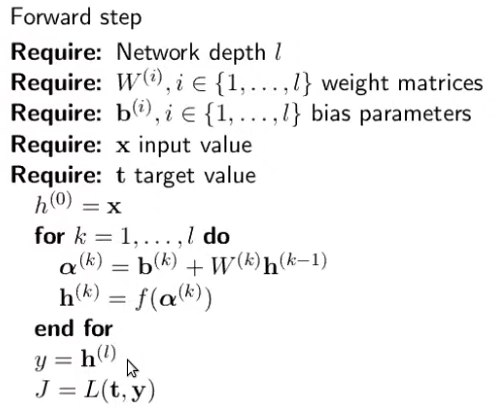
\includegraphics[width=15cm]{images/FNN/backprop_forward_Step.png}
    \caption{Forward step}
    \label{fig:forw_step}
\end{figure}

\begin{figure}[H]
    \centering
    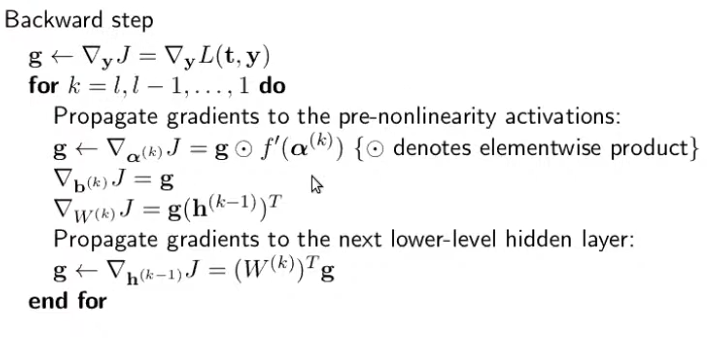
\includegraphics[width=15cm]{images/FNN/backprop_backward_Step.png}
    \caption{Backward step}
    \label{fig:backw_step}
\end{figure}

\textbf{Note}: this algorithm is specific for MLPs. This algorithm can also be optimized through caching.

\subsection{Learning Algorithms}
\subsubsection{SGD}

\begin{figure}[H]
    \centering
    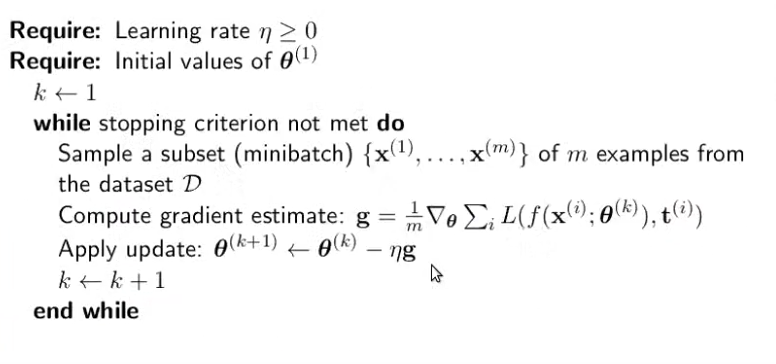
\includegraphics[width=15cm]{images/FNN/SGD.png}
    \caption{SGD algorithm. The gradient is calculated through the backpropagation.}
    \label{fig:sgd}
\end{figure}

We change $\eta$ according to some rules through iterations.

Until iteration $\tau$:
\begin{equation}
    \eta^{(k)} = \left(1 - \frac{k}{\tau}\right)\eta^{(k)} + \frac{k}{\tau}\eta^{(\tau)}
\end{equation}
after iteration $\tau$ we have $\eta^{(k)} = \eta^{(\tau)}$

\subsubsection{SGD with momentum}
\begin{figure}[H]
    \centering
    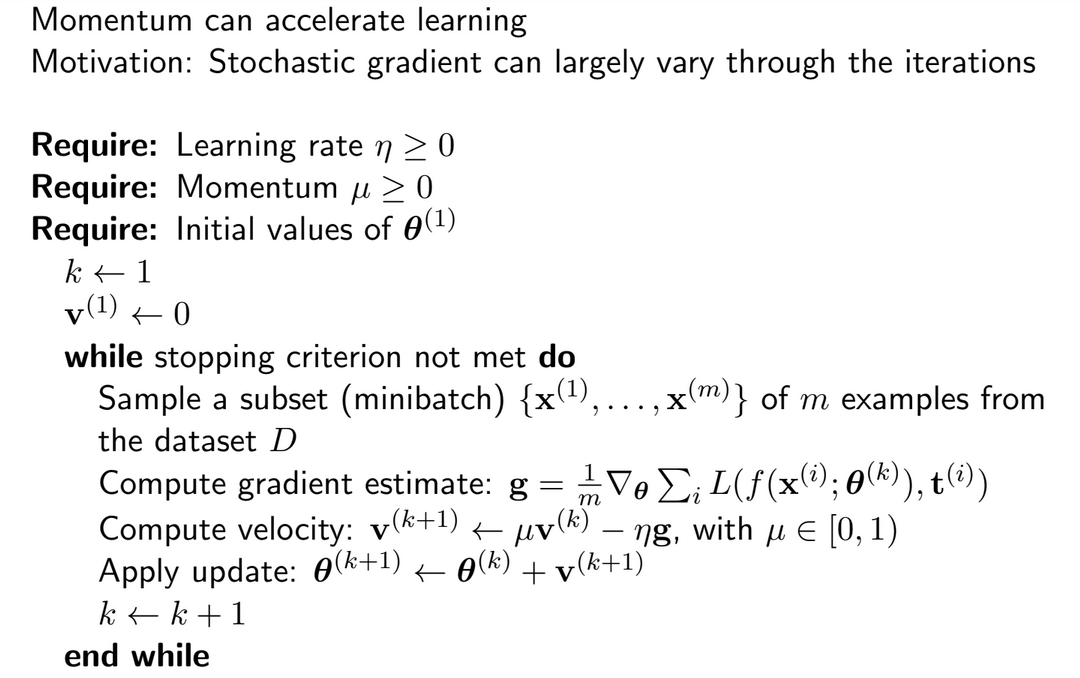
\includegraphics[width=15cm]{images/FNN/SGD_momentum.png}
    \caption{SGD algorithm with momentum. The gradient is calculated through the backpropagation.}
    \label{fig:sgd_momentum}
\end{figure}
Momentum helps overcome local minimums. It starts an oscillation movement when he reaches a minimum.

SGD with \textbf{Nestov} momentum is another technique that consists in applying the momentum before computing the gradient. This technique sometimes improves the convergence rate.

\subsubsection{Adaptive learnings}
Based on th eanalisys of the gradient of the loss function it's possible to determine, at any step algorithm, whether the learning rate should be increased or decreased.

Some examples of adaptive learning rates are:
\begin{itemize}
    \item AdaGrad
    \item RMSProp
    \item Adam
\end{itemize}


\subsection{Architectural Design}
What can we chose of a FNN?
\begin{itemize}
    \item Depth
    \item Width of a layer
    \item Activation functions
    \item Loss function
\end{itemize}

The \textbf{Universal Approximation Theorem} does not say how to set these parameters.

For the output of the neural network we can use the softmax if we have to classify the datapoint. The softmax will be translated into a one-hot encoding ({1, 0, 0}, {0, 1, 0}, ...) or in a Categorical encoding ({1, 2, 3}).\\
for the loss function we have two formats of the output: Categorical Cross Entropy vs Sparse categorical cross entropy.

How do we calculate the number of parameters for a Fully connected layer?
if we have $a$ layers as input and the next layer has $b$ units we can calculate the number of parameters as: $a \times b + b = (a + 1) \times b$. We can calculate the number of parameters for each Fully connected layer and sum the values to get the total number of parameters.



\subsection{Regularization}
Regularizatoin is an important step for FNN too if we want to reduce overfitting.\\
We have different options for FNN:
\begin{itemize}
    \item Parameter norm penalties
    \item Dataset argumentation
    \item Early stopping
    \item Parameter sharing
    \item Dropout
\end{itemize}

If the network improves the accuracy on Training set but not on Test set then the network is overfitting.

\subsubsection{Parameter norm penalties}
We can penalize high absolute values of the parameters:
\begin{equation}
    E_{reg}(\Theta) = \sum_{j} |\Theta_{j}|^{q}
\end{equation}
resulting in the cost function:
\begin{equation}
    \overline{J}(\Theta) = J(\Theta) + \lambda E_{reg}(\Theta)
\end{equation}

Programming Libraries usually let you choose a $\lambda$ for each layer. If the value is not set, il will be set to $0$ and the parameters will not be penalized.

\subsubsection{Dataset Argumentation}
We can generate new datapoint and include them in the dataset.
\begin{itemize}
    \item Data Transformation
    \item Adding noise
\end{itemize}

\subsubsection{Early Stopping}
We can stop iterations early to avoid overfitting. In order to know when to stop we can use cross-validation to determine the best values. We can also send different training run with random initialization values, where each run will evolve differently an maybe one of them will have a better accuracy.

\subsubsection{Parameter sharing}
Parameter sharing consists in setting constraints on having subset of model parameters to be equal.

In CNNs this method allows for invariance to translation.

\subsubsection{Dropout}
Randomly ignore network units with some probability $\alpha$. So I will apply the algorithm only on a subset of connection (for a single step). I can apply dropout to every step an randomly ignore a different random subset of parameters at each iteration.

\subsection{Convolutional Neural Networks}

\subsection{Motivation}
Up to now we treated inputs as general feature vectors. In some cases they have a special structure:
\begin{itemize}
    \item Audio
    \item Images
    \item Videos
\end{itemize}

Signals are a numerical representation of physical quantities. Deep learning can be directly applied on signals by using suitable operations.

We cannot simply flatten the input because images, audio and videos have a semantics that cannot be ignored. By flatting the input we loose information and consequently the network will not behave well.

\subsubsection{Convolution}
Given an image $I$ and a kernel $K$, the 2-D convolution is:
\begin{equation}
    (I*K)(i,j) \equiv \sum_{m \in S_{1}}\sum_{n \in S_{2}} I(m, n)K(i-m, j-n)
\end{equation}
where $S_{i}$ are finite sets.
for a 3-D convolution the formula is:
\begin{equation}
        (I*K)(i,j, k) \equiv \sum_{m \in S_{1}}\sum_{n \in S_{2}}\sum_{u \in S_{3}} I(m, n, u)K(i-m, j-n, k-u)
\end{equation}
Properties: 
\begin{itemize}
    \item convolution is commutative: $(I*K)(i, j) = (K*I)(i, j)$
    \item Cross-correlation: we can flip the kernel and modify the convoution
    \begin{equation}
        (I*K)(i,j) \equiv \sum_{m \in S_{1}}\sum_{n \in S_{2}} I(i+m, j+n)K(m, n)
    \end{equation}
\end{itemize}

\subsubsection{Different types of Convolution}
based on the direction of the movement of the kernel, the convolution can be 1D, 2D, 3D...\\
So it is based on the degree of freedom of the kernel.

Convolution changes the shape of the tensor.

\subsubsection{Padding}
We can add a padding in order to convolve and keep the size of the image. Padding can be all zeros

\subsection{Terminology}
\begin{itemize}
    \item Input size
    \item Kernel size
    \item Feature map or Depth slice: output of convolution between an input and one kernel
    \item Depth: number of kernels
    \item Padding
    \item Stride: step of sliding kernel
    \item Receptive field: region in the input space that a particular feature is looking at.
\end{itemize}

\subsubsection{Convolutional Layers}
Are usually made up by three layers:
\begin{itemize}
    \item Convolution between input and kernel
    \item non-linear activation function
    \item pooling
\end{itemize}

For the detector stage we use one of the same that we use for FNNs.

\subsubsection{Properties of CNNs}
Sparse interaction/connectivity: brings in the concept of locality.
Parameter sharing: constraint on values of the kernels.

Pooling stage implements invariance to local translations. Some frequently used pooling layers are \textbf{maxpooling} and \textbf{average pooling}. When applied with stride it reduces the size of the output layer (\textbf{subsampling}).

\subsubsection{Calculate the feature map size}
Consider the input size $w_{in} \times h_{in} \times d_{in}, d_{out}$ kernels of size $w_{k} \times h_{k} \times d_{in}$, stride $s$ and padding $p$, the dimension of the feature map can be calculated as:
\begin{equation}
    w_{out} = \frac{w_{in} - w_{k} + 2p}{s} + 1
\end{equation}
\begin{equation}
    h_{out} = \frac{h_{in} - k_{k} + 2p}{s} + 1
\end{equation}

while the number of trainable parameters is: 
\begin{equation}
    |\Theta| = w_{k} \cdot h_{k} \cdot d_{in} \cdot d_{out} + d_{out}
\end{equation}

\subsection{Networks for Images}

\textbf{}{LeNet} is a simple but yet good neural network composed of 7 layers.
The input is a $32 \times 32$ image and the output are 10 neurons (10 classes).

Other famous neural networks (not deep) are:
\begin{itemize}
    \item ResNet
    \item VGG
    \item GoogLeNet
    \item AlexNet
\end{itemize}

\subsection{Transfer Learning}
The idea is to understand how to exploit learning on a different task for learning on a new task.\\
$D$ is a domain defined by data points $x_{i} \in X$, distributed according to $D(X)$. $T$ is a learning task defined by labels $y \in Y$, a target function $f: X \xrightarrow[]{} Y$, and distribution $P_{D}(y|x)$.\\
Given:
\begin{itemize}
    \item $D_{T}$ and $T_{S}$ a source domain learning task
    \item $D_{T}$ and $T_{T}$ a target domain learning task
    \item in general $D_{S} \neq D_{T}$ and $T_{S} \neq T_{T}$
\end{itemize}
Our goal is to improve learning of $f_{T}: X_{T} \xrightarrow[]{} Y_{T}$ using knowledge in $D_{S}$ and $DT_{S}$.

\subsubsection{Solutions}
\textbf{Fine-tuning}: Use the same architecture (or part of it) and initialize it with the pretrained models. Then you can:
\begin{itemize}
    \item train of all network parameters
    \item freeze parameters of some layers.
    \begin{itemize}
        \item \textbf{Pros}: Full advantage of CNNs.
        \item \textbf{Cons}: 'Heavy' training.
    \end{itemize}
\end{itemize}

\textbf{CNN as feature extractor}: We use a CNN as a feature extractor network, usually by cutting the last layers and by then using a flatten/dense layer. Then we train a new classifier based on those extracted features.
\begin{itemize}
        \item \textbf{Pros}: No need to train CNNs.
        \item \textbf{Cons}: Cannot modify features
\end{itemize}
